%%%%%%%% ICML 2019 EXAMPLE LATEX SUBMISSION FILE %%%%%%%%%%%%%%%%%

\documentclass{article}

% Recommended, but optional, packages for figures and better typesetting:
\usepackage{microtype}
\usepackage{graphicx}
\usepackage{subfigure}
\usepackage{booktabs} % for professional tables

% hyperref makes hyperlinks in the resulting PDF.
% If your build breaks (sometimes temporarily if a hyperlink spans a page)
% please comment out the following usepackage line and replace
% \usepackage{icml2019} with \usepackage[nohyperref]{icml2019} above.
\usepackage{hyperref}

% Attempt to make hyperref and algorithmic work together better:
\newcommand{\theHalgorithm}{\arabic{algorithm}}

% Use the following line for the initial blind version submitted for review:
\usepackage{icml2019}
\newcommand{\bg}[1]{~{{[{\it \textcolor{red}{{\bf BG:} #1}}]}}}
\newcommand{\cs}[1]{~{{[{\it \textcolor{red}{{\bf CS:} #1}}]}}}
\newcommand{\ag}[1]{~{{[{\it \textcolor{red}{{\bf AG:} #1}}]}}}
% If accepted, instead use the following line for the camera-ready submission:
%\usepackage[accepted]{icml2019}

% The \icmltitle you define below is probably too long as a header.
% Therefore, a short form for the running title is supplied here:
\icmltitlerunning{Submission and Formatting Instructions for ICML 2019}

\begin{document}

\twocolumn[
\icmltitle{Submission and Formatting Instructions for \\
           International Conference on Machine Learning (ICML 2019)}

% It is OKAY to include author information, even for blind
% submissions: the style file will automatically remove it for you
% unless you've provided the [accepted] option to the icml2019
% package.

% List of affiliations: The first argument should be a (short)
% identifier you will use later to specify author affiliations
% Academic affiliations should list Department, University, City, Region, Country
% Industry affiliations should list Company, City, Region, Country

% You can specify symbols, otherwise they are numbered in order.
% Ideally, you should not use this facility. Affiliations will be numbered
% in order of appearance and this is the preferred way.
\icmlsetsymbol{equal}{*}

\begin{icmlauthorlist}
\icmlauthor{Aeiau Zzzz}{equal,to}
\icmlauthor{Bauiu C.~Yyyy}{equal,to,goo}
\icmlauthor{Cieua Vvvvv}{goo}
\icmlauthor{Iaesut Saoeu}{ed}
\icmlauthor{Fiuea Rrrr}{to}
\icmlauthor{Tateu H.~Yasehe}{ed,to,goo}
\icmlauthor{Aaoeu Iasoh}{goo}
\icmlauthor{Buiui Eueu}{ed}
\icmlauthor{Aeuia Zzzz}{ed}
\icmlauthor{Bieea C.~Yyyy}{to,goo}
\icmlauthor{Teoau Xxxx}{ed}
\icmlauthor{Eee Pppp}{ed}
\end{icmlauthorlist}

\icmlaffiliation{to}{Department of Computation, University of Torontoland, Torontoland, Canada}
\icmlaffiliation{goo}{Googol ShallowMind, New London, Michigan, USA}
\icmlaffiliation{ed}{School of Computation, University of Edenborrow, Edenborrow, United Kingdom}

\icmlcorrespondingauthor{Cieua Vvvvv}{c.vvvvv@googol.com}
\icmlcorrespondingauthor{Eee Pppp}{ep@eden.co.uk}

% You may provide any keywords that you
% find helpful for describing your paper; these are used to populate
% the "keywords" metadata in the PDF but will not be shown in the document
\icmlkeywords{Machine Learning, ICML}

\vskip 0.3in
]

% this must go after the closing bracket ] following \twocolumn[ ...

% This command actually creates the footnote in the first column
% listing the affiliations and the copyright notice.
% The command takes one argument, which is text to display at the start of the footnote.
% The \icmlEqualContribution command is standard text for equal contribution.
% Remove it (just {}) if you do not need this facility.

%\printAffiliationsAndNotice{}  % leave blank if no need to mention equal contribution
\printAffiliationsAndNotice{\icmlEqualContribution} % otherwise use the standard text.

\begin{abstract}

A goal of probabilistic programming is to couple simulators, with inference. This is 
because stochastic simulators are used prominently in many industrial settings,
do not require one to construct hand-crafted joint distributions as they implicitly 
define a joint distribution of the program and encode learnt structures 
directly. This makes simulators powerful tools and much of machine learning (ML) and 
Artificial Intelligence (AI)
can be seen as trying to emulate such simulators from a purely data-driven approach.
However, in the 
ML/AI setting, although we can often infer outcomes, we have little understanding about what 
in the data led to the outputted inferences. 
This makes it challenging to deploy ML/AI systems into the wild, especially in health-related and safety-critical domains, such
as epidemiology, as we lose \emph{interpretability}. 
In this work, we explain how to design ML/AI systems that combine
probabilistic programming systems (PPSs) and epidemiology simulators, to extract
fully interpretable posterior structures, enabling policy makers 
and practitioners to make interpretable inferences. 
In particular, we demonstrate this for the Malaria disease and show how we can 
perform interpretable inference in such settings.
\end{abstract}

\section{Introduction}

To do. 

\begin{itemize}

\item Outline the objectives
\item State the importance of interpretability in the inference of the simulator
\item Our system enables one to understand and interpret the most common paths in a program (simulation).
\item In highlighting this a practitioner can then go back to the field and explore that parameter/s in more depth.
\item This facilitates understanding and the construction of more detailed models and data collection strategies


\end{itemize}

% taken from Toms thesis. 

Stochastic simulators are common across a number of domains, statistical physics~\cite{landau_binder_2014}, financial modeling~\cite{jackel2002monte},
weather prediction~\cite{evensen1994sequential}, epidemiology~\cite{smith2008towards} and many others. 
An advantage of using stochastic simulators is that they provide a level of interpretability not found in modern deep learning settings, as they directly incorporate model structure from carefully reasoned observations and experiments.  
Probabilistic programming systems~(PPSs) are purpose built systems for making inferences and probabilistic 
modeling accessible. 
In particular, PPSs allow probabilistic models to be represented in the form of a generative model through the
probabilistic programming language~(PPL), which enables one to write statements that enable conditioning on data~\cite{gordon2014probabilistic,Goodman08church:a}. 
Thus, it seems only natural to connect simulators with PPSs, as simulators explicitly define a generative model, in the language in which they are written, and the nature of the PPSs enables us to perform inference in these simulators, by conditioning on observations, which are fed in as input to the simulators. 
In doing this we can infer things about stochastic input parameters and other variables sampled during the program's forward execution, whilst also providing full interpretability in the inference results, which is absolutely necessary in safety-critical domains.
By exploiting the tools that we develop in this paper, one is able to connect epidemiology simulators with \texttt{Pyprob}~\cite{le-2016-inference} to extract fully interpretable posterior structures allowing practitioners to interpret which input parameters have the largest affect on the epidemic, in our case malaria. Over five-hundred-thousand people die from malaria each year, mostly children under five years of age, with 90 per cent of malaria cases occurring in Sub-Saharan Africa. An estimated 100-300 million people suffer from malaria each year~\cite{world2016world}. 
Thus, by understanding the prominence of input parameters to epidemiology simulators, guides decision making processes relating to effective treatment and prevention strategies. 
\label{sec:related}


\section{Epidemiology Simulators and Probabilistic Programming}
\label{sec:background}
This will kind of be like a background section. 



\section{Methodology}

\subsection{Probabilistic Programming}
Probabilistic programming~\cite{gordon2014probabilistic,staton2016semantics,kozen1979semantics} is the coming together of multiple disciplines; computer science, statistics and machine learning. 
It attempts to unify the three fields by creating automated frameworks in which one can easily extrapolate their observed data and perform sophisticated statistical analysis with advance inference procedures such as 
Markov Chain Monte Carlo (MCMC), Variational Inference~(VI) and Deep Neural Networks~(DNN) in an accessible way, i.e. without the need of expert knowledge in implementing and using such procedures.
Users can then exploit these algorithms on an array of models
within the probabilistic programming language~(PPL), using the language itself to create models that represent complicated distribution objects. 
PPLs typically extend existing programming languages such as python, c++, go and so forth, which means that users do not have to learn
a completely new set of operating semantics.  
Our PPL PyProb~\cite{le-2016-inference,baydin2018efficient} belongs to the family of universal PPLs 
that allow the expression of unrestricted probability models in a Turing complete fashion~\cite{wood2014new,goodman2012church,landau_binder_2014,siddharth2017learning,bingham2019pyro}.

\subsection{Stochastic Simulators}

Simulators encode several years, if not decades, of research and development and so by their very nature are structurally complicated. Within the context of epidemiology simulators we can model treatment, infection and prevention cycle under a variety of different environmental conditions, enabling predictions to be made given a series of field observations \bg{Make sure that I do not state they can already do what PP can do, i.e. the ability to update and infer the input parameters continually conditioned on new observations.}. However, since the development happens over several decades, usually without comprehensive documentation, understanding a code base written with legacy libraries and software is incredibly difficult and an almost impossible task for a non-expert, or expert who has not had access to the previous years of development. Our method of hijacking simulators builds on the work of~\cite{baydin2018efficient} and extends the framework to encapsulate a more diverse range of simulators. Our framework provides a simple solution and makes it easy to transform arbitrary stochastic simulators into probabilistic programs, regardless of the complexity of the simulator and the language that the simulator is written in\footnote{The framework currently supports 9 popular languages, but there is nothing to stop this being extended to any language of interest.}. In addition to this, we can understand the structure of programs in simulators for both decoding \emph{black-box structures} and for posterior inference. This enables two things. 1) It enables software developers and researchers to understand complicated code bases. 2) It provides interpretable inference results that provide policy makers with predictions that are truly interpretable, in the sense that the end-user of the inference results understands what physical events led to inference outcome. This is critical in several domains, and is particularly important in the medical domain. We provide examples of former in next Section~\textbf{TO ADD REF} and discuss the latter in ~\bg{Link to conclusion / future work}.


\section{Case Study}
\subsection{Connecting a Stochastic Simulator to a Probabilistic Programming System}

In order to hijack the stochastic simulator we are only required to override the location of the stochastic primitives, i.e. the operations that generate the stochasticity and randomness within the simulator. 
We will walk through how this is done for EMOD and OpenMalaria, you will see that it is procedurally identical.
However, given the sheer number of simulators it maybe slightly different procedurally. 
To our knowledge it shouldn't be, but we have not been able view of all stochastic simulators we cannot make this guarantee with certainty. 
The first step is to build a containerized environment, such as Docker~\cite{merkel2014docker} and Singularity~\cite{kurtzer2017singularity}, which enables the simulators to be run on any device, independent of different hardware architectures, removing the requirement for hardware specific machines. 
This greatly improves the scope of applicability of our system, as this environment only has to be built once, which then enables the simulator to be run simultaneously on machines of different architectures machine. 
The second step requires one to 


% \subsection{Extending Probabilistic Programming Protocols}

\begin{figure*}[h!]
	\centering
	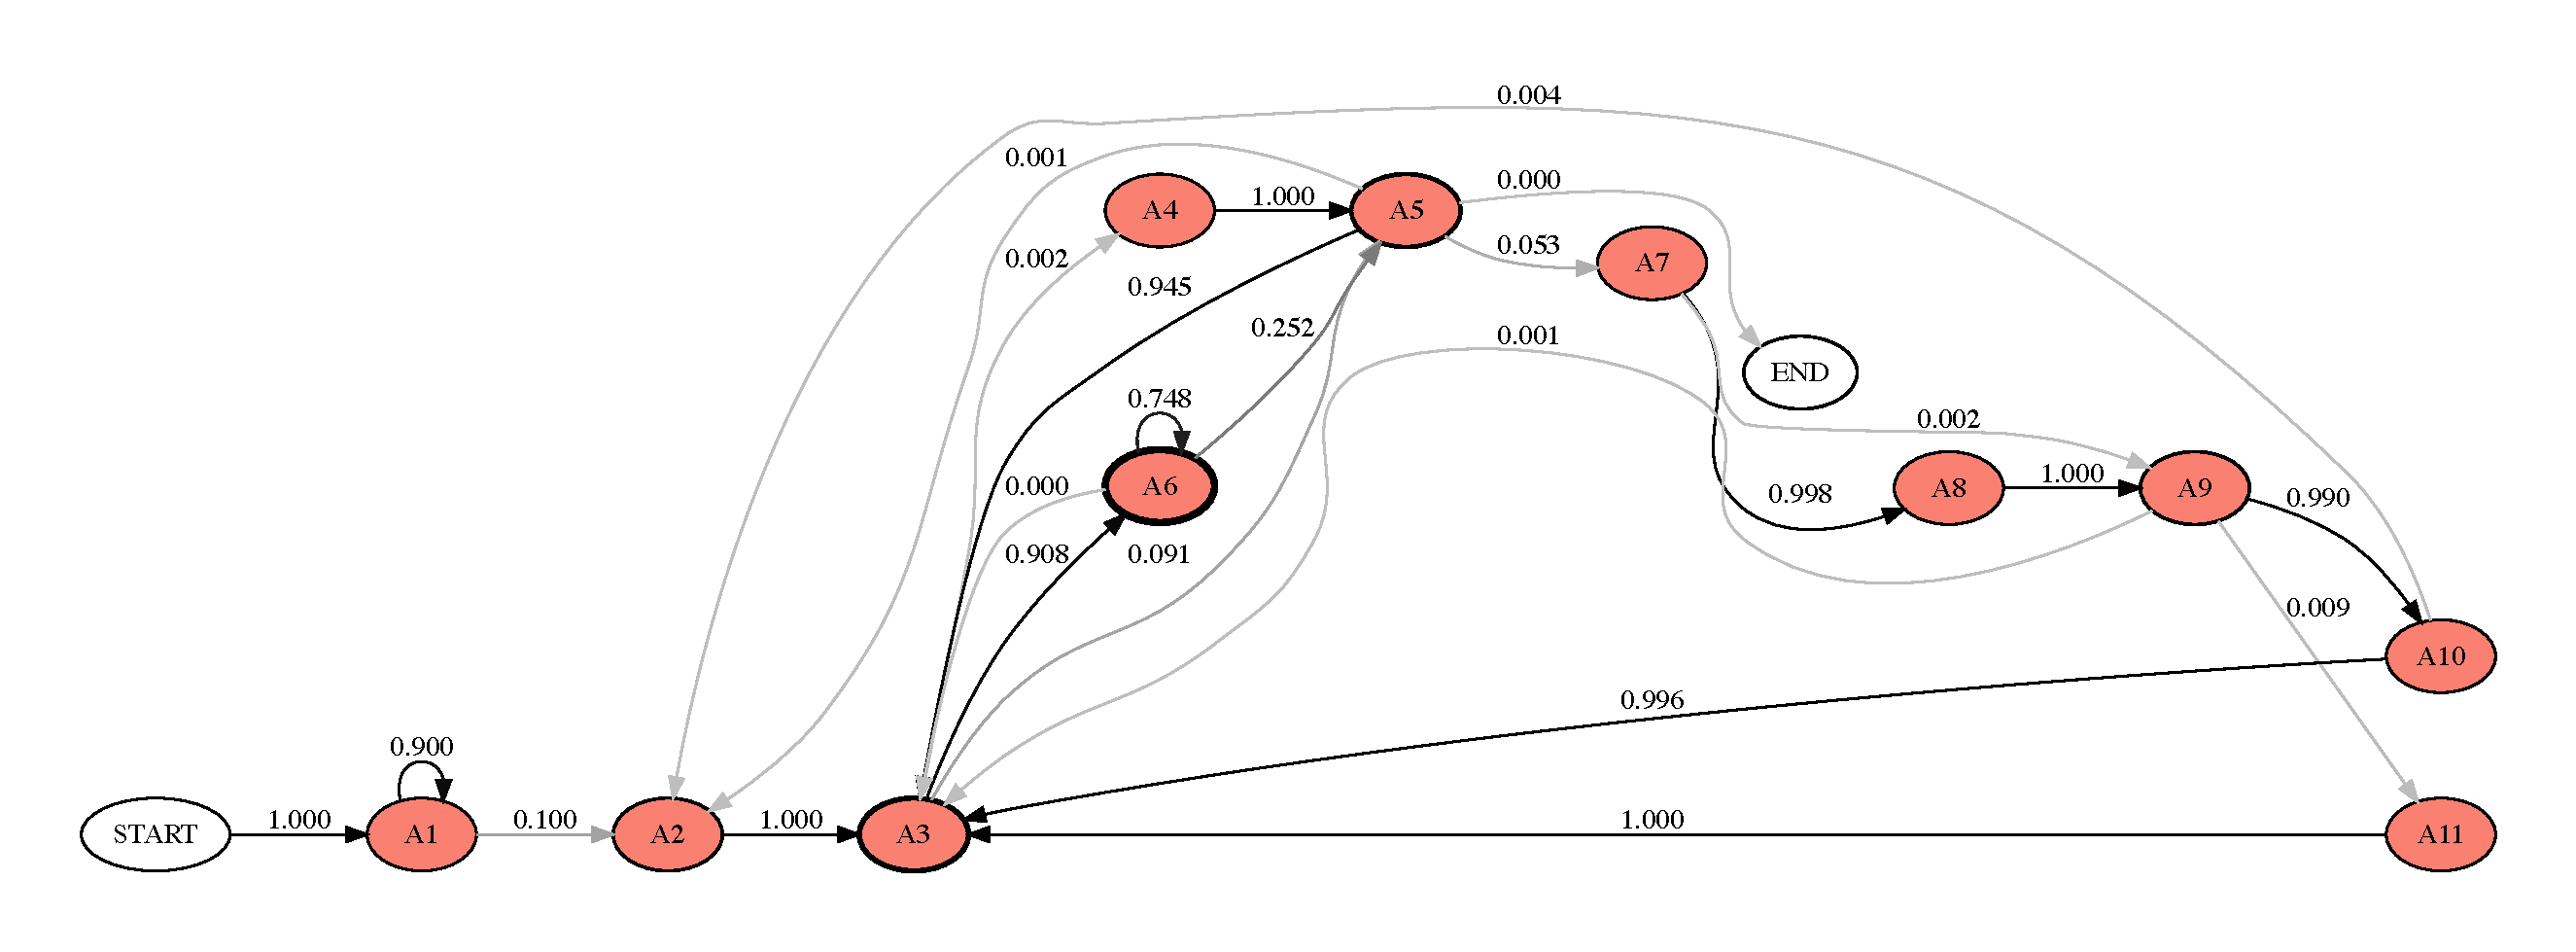
\includegraphics[width=\textwidth]{../plots/ewan_25_pop_10.pdf}
	\caption{Add something. Population 10}
\end{figure*}
\begin{figure*}[h!]
	\centering
	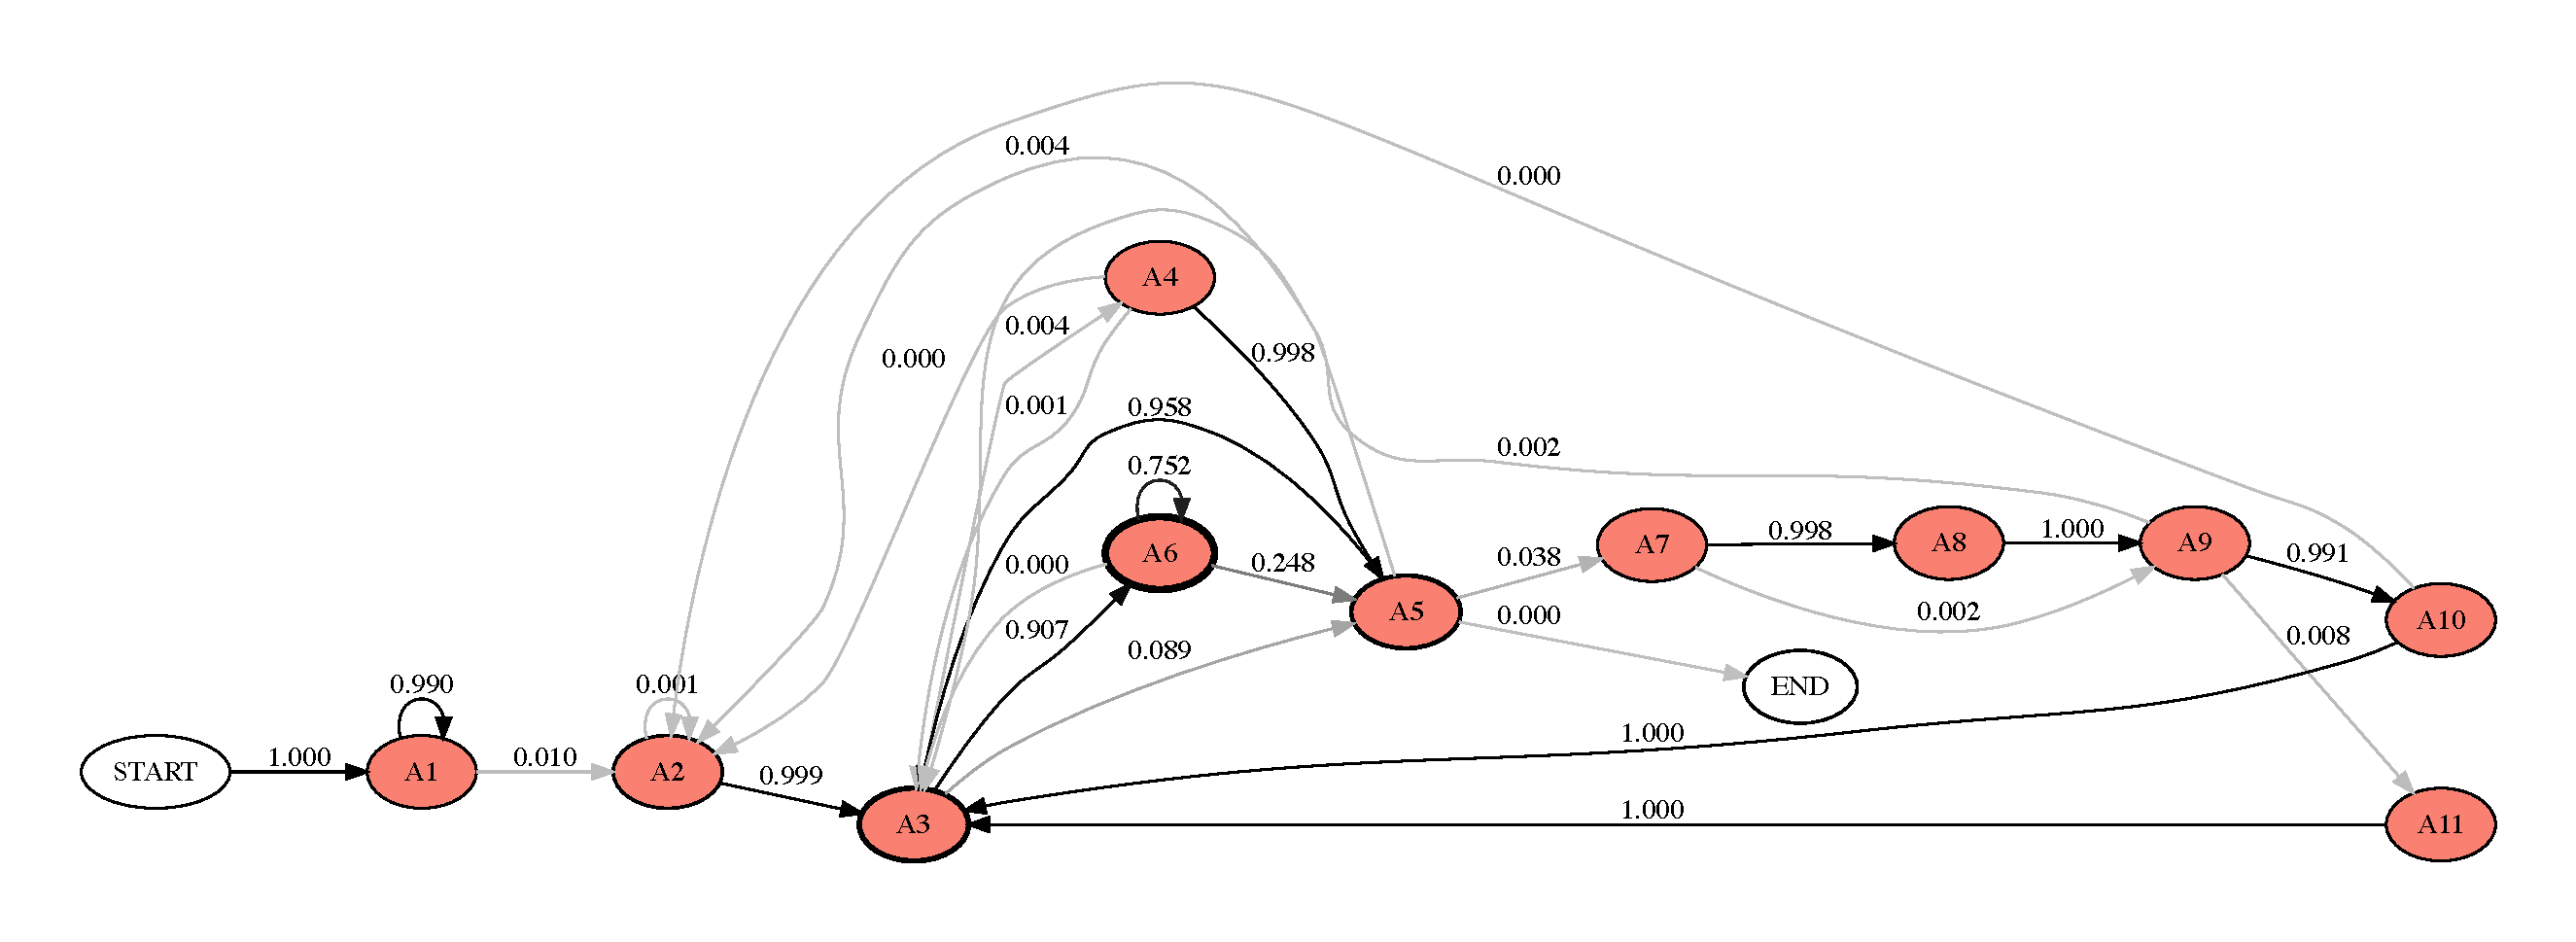
\includegraphics[width=\textwidth]{../plots/ewan_25_pop_100.pdf}
	\caption{Add something. Population 100}
\end{figure*}
TODO

\section{Results}

TO ADD


% \subsubsection*{Acknowledgments}

% Use unnumbered third level headings for the acknowledgments. All acknowledgments
% go at the end of the paper. Do not include acknowledgments in the anonymized
% submission, only in the final paper.

\section*{References}

\bibliographystyle{icml2019}
\bibliography{refs}

\end{document}


% This document was modified from the file originally made available by
% Pat Langley and Andrea Danyluk for ICML-2K. This version was created
% by Iain Murray in 2018, and modified by Alexandre Bouchard in
% 2019. Previous contributors include Dan Roy, Lise Getoor and Tobias
% Scheffer, which was slightly modified from the 2010 version by
% Thorsten Joachims & Johannes Fuernkranz, slightly modified from the
% 2009 version by Kiri Wagstaff and Sam Roweis's 2008 version, which is
% slightly modified from Prasad Tadepalli's 2007 version which is a
% lightly changed version of the previous year's version by Andrew
% Moore, which was in turn edited from those of Kristian Kersting and
% Codrina Lauth. Alex Smola contributed to the algorithmic style files.
